\subsection{Häufigkeitsverteilung}
Hinweis zur Notation: $x_m^u$ bedeutet, das (kleine) $x$ aus der Klasse $m$, das $u$ steht für die Untere Grenze einer Klasse. 
\subsubsection{Mittelwerte}
\begin{itemize}
	\item Dichte: Die Dichte sagt aus, wie viel der Grundgesamtheit innerhalb der gewählten Klasse sind
	\begin{equation}\label{theorie:mittelwerte:dicht}
	d_j = \frac{h_j}{x_j^o-x_j^u}
	\end{equation}
	\item Modus: Der Modus ist derjenige Merkmalswert, der am häufigsten beobachtet wird %BILD
	\begin{equation}\label{theorie:mittelwerte:modus:1}
	M_{o}=x_{m}^{u}+\frac{h_{m}-h_{m-1}}{(h_{m}-h_{m-1})+(h_{m}-h_{m+1})}\cdot(x_{m}^{o}-x_{m}^{u})
	\end{equation}
	\item Modus bei unterschiedlichen Klassengrössen
	\begin{equation}\label{theorie:mittelwerte:modus:2}
	M = x_m^u + \frac{d_m-d_{m-1}}{(d_m-d_{m-1})+(d_m-d_{m+1})}
	\end{equation}
	\item Quantile: Ein Quartil ist ein Merkmals wert durch den die Gesamtheit in zwei Teile zerlegt\\
	Ansatt $\frac{1}{2} n$ wird $\frac{3}{4} n$ genommen:\\
	\begin{eqnarray}\label{theorie:mittelwerte:quant}
	M_{e}=x_{m}^{u}+\frac{\frac{n}{2}-H_{m-1}}{(H_{m}-H_{m-1})}\cdot(x_{m}^{o}-x_{m}^{u})
	\end{eqnarray}
	Die Formel des Medians ist diesselbe Formel wie die fürs zweite Quantil(hier beschrieben)
	\item Arithmetisches Mittel: Das arithmetische Mittel ist der Wert, der sich bei gleichmässiger Verteilung der Summe aller beobachteten Merkmalswerte auf alle Merkmalsträger ergibt.\\
	Nicht klassifizierte berechnung:
	\begin{eqnarray} \label{theorie:mittelwerte:arith}
	\overline{x}&=&\frac{1}{n}\sum_{i=1}^{v}x_i\cdot h_i\\
	\overline{x}&=&\sum_{i=1}^{v}x_i\cdot f_i\\
	\end{eqnarray}
	\item Harmonisches Mittel: Das harmonische Mittel ist derjenige Wert, zu dem die in der Häufigkeitsverteilung vor ihm liegende Merkmals werte in der Summe gesehen relativ gleich weit entfernt sind wie die nach ihm liegenden Merkmals werte
	\begin{eqnarray}\label{theorie:mittelwerte:harmo}
	\overline{MH}=\frac{\sum_{i=1}^{v}h_i}{\sum_{i=1}^{v}\frac{h_i}{x_i}}
	\end{eqnarray}
	\item Geometrisches Mittel: Das geometrische Mittel ist die n-te Wurzel aus dem Produkt aller beobachteten Merkmals werte.%BILD
	\begin{eqnarray}\label{theorie:mittelwert:geome}
	MG=\sqrt[n]{\prod_{i=1}^{n}x_i}=\sqrt[n]{\frac{\mbox{endwert}}{\mbox{anfangswert}}}\longrightarrow \sqrt[3]{\frac{57}{40}}=1.125
	\end{eqnarray}
	\item Binominalkoeffizient: Dieser wird verwendet, wenn man mögliche Kombinationen berechnen möchte. 
    \begin{equation}
    {n \choose k} = \frac{n!}{k!(n-k)!} \Rightarrow {18 \choose 3} = \frac{18\cdot17\cdot16}{3!}
    \end{equation}
\end{itemize}
Weitere Informationen gibt es im \autoref{praxis:mittelwerte}
\subsubsection{Spannweite}
\begin{itemize}
	\item Spannweite: Die Spannweite $R$ ist die Differenz aus dem grössten und dem kleinsten beobachteten Merkmalswert.
	\begin{eqnarray}
	R&=&\mbox{grösster Merkmalswert}-\mbox{kleinster Merkmalswert}\\
	R&=&x[n]-x[1]\\
	\end{eqnarray}
	Klassifizierte Häufigkeitsverteilung
	\begin{eqnarray}
	R=x_{v}^{o}-x_{1}^{u}
	\end{eqnarray}
	\item Zentralen Quartilsabstand: Der zentrale Quartislabstand ist die Entfernung zwischen den beiden Merkmalswerten, welche die in der Rangordnung zentral gelegenen 50\% der Merkmalsträger eingrenzen.
	%BILD
	\begin{eqnarray}
	ZQA=Q_3-Q_1
	\end{eqnarray}
	\pagebreak[4]
	\item Mittlere absolute Abweichung: Die mittlere absolute Abweichung ist die durchschnittliche Entfernung aller beobachteten Merkmalswerte von arithmetischen Mitteln (alternativ: Median)
	\begin{eqnarray}
	\delta= \frac{1}{n}\cdot \sum_{i=1}^{v}\cdot \vert x_i - \overline{x} \vert \cdot h_i
	\end{eqnarray}
	\begin{itemize}
		\item $n$: Anzahl Merkmalsträger
		\item $v$: Anzahl der verschiedenen Merkmalswerte
		\item $h_i$: Absolute einfache Häufigkeit der an Merkmalsträger mit dem Merkmalswert: $x_i$
	\end{itemize}
	\item Varianz und Standardabweichung: Die Varianz ist die SUmme der quadrierten Abweichungen der Merkmalswerte vom arithmetischen Mittel, dividiert durch die Anzahl der Merkmalsträger. Die Standardabweichung ist die Quadratwurzel aus der Varianz
	\begin{eqnarray}
	\sigma^{2}=\frac{1}{n}\sum_{i=1}^{n}(x_i-\overline{x})^2 h_i
	\end{eqnarray}
	\item Variationskoeffizienten: Der Variationskoeffizient misst nicht die absolute, sondern die relative Streuung. Das heisst, er setzt die Streuung in Relation zur Lage der Häufigkeitsverteilung. Der Variationskoeffizient ist der Quotient aus Standardabweichung und arithmetischem Mittel, multipliziert mit 100
	\begin{eqnarray}
	VK=\frac{\sigma}{\overline{x}}\cdot 100
	\end{eqnarray}
\end{itemize}
\pagebreak[2]
\subsubsection{Boxplot}
Ein Boxplot stellt die Verteilung kardinalskalierter Daten dar, fasst verschiedene robuste Streuungs- und Lagemasse in einer Darstellung zusammen. Es vermittelt schnell einen Eindruck, in welchem Bereich die Daten liegen und wie sie sich über diesen Bereich verteilen.
\begin{figure}[htb]
\centering
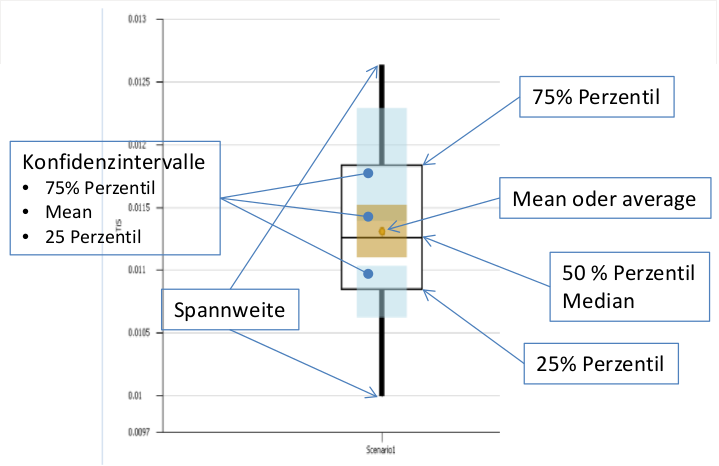
\includegraphics[scale=0.5]{images/exev_haufigkeitsverteilung_boxplot_1.png}
\caption{Boxplot Beispiel}
\label{fig:theory:boxplot:1}
\end{figure}
